\documentclass[12pt,a4paper]{article}
\usepackage{fancyhdr}
\usepackage{fontspec}
\usepackage{amsmath}
\usepackage{amssymb}
\usepackage{bm}
\usepackage{tikz}
\setmainfont{Microsoft YaHei}
\pagestyle{fancy}

\begin{document}

\fancyfoot[C]{by chinasjtu@msn.com }

\newcommand{\nl}{\newline}

\newcommand{\ntinf}{\lim\limits_{n \to \infty}}
\newcommand{\xtinf}{\lim\limits_{x \to \infty}}

\newcommand{\Atinf}{\lim\limits_{A \to \infty}}
\newcommand{\Rtinf}{\lim\limits_{R \to \infty}}

\newcommand{\ntx}[1]{\lim\limits_{n \to #1}}
\newcommand{\xtx}[1]{\lim\limits_{x \to #1}}
\newcommand{\ttx}[1]{\lim\limits_{t \to #1}} 
\newcommand{\ktx}[1]{\lim\limits_{k \to #1}} 
\newcommand{\dxtx}[1]{\lim\limits_{\Delta x \to #1}}

\newcommand{\jfab}{\int_{a}^{b}}
\newcommand{\jf}[2]{\int_{#1}^{#2}}

\newcommand{\nsum}[2]{\sum\limits_{n=#1}^{#2}}
\newcommand{\isum}[2]{\sum\limits_{i=#1}^{#2}}
\newcommand{\ksum}[2]{\sum\limits_{k=#1}^{#2}}

\newcommand{\nsuminf} {\nsum{1}{\infty}}
\newcommand{\ksuminf} {\ksum{1}{\infty}}
\newcommand{\isuminf} {\isum{1}{\infty}}




\begin{center} 第12章 Fourier级数  \end{center}

$\frac{a_0}{2}+\nsuminf (a_ncosnx+b_nsinnx)~f(x)$

$f(x) g(x) \in C[a,b]<f,g>=\jf{a}{b}fgdx$

$<f_i(x),f_j(x)>=
\begin{cases} 0, i \ne j \\ \lambda_i, i=j \end{cases}$

$例:1,cosx,sinx,cos2x,sin2x,...coskx,sinkx$

$在[c,c+2\pi](c \in R)上的正交系,在[0,\pi]上不正交$

$1,cosx,cos2x,....与sinx,sin2x,...均为正交系,在[0,\pi]上$

$一般地1,cos\frac{\pi x}{l},sin\frac{\pi x}{l},...,cos\frac{k\pi x}{l},sin\frac{k\pi x}{l}为[0,2l]或$

$[-l,l]上正交系,而\frac{1}{\sqrt{2l}},\frac{1}{\sqrt{l}}cos\frac{\pi x}{l},\frac{1}{\sqrt{l}}sin\frac{\pi x}{l},...为标准正交基$

$\nl$

$将周期为2\pi 的函数,f(x)= \begin{cases} -\pi, -\pi<x<0 \\ x, 0\le x<\pi \end{cases}展开为付氏级数$

$a_0=\frac{1}{\pi}(\jf{-\pi}{0}-\pi dx+\jf{0}{\pi}xdx)=-\frac{1}{2}\pi$

$a_n=\frac{1}{\pi}(\jf{-\pi}{0}-\pi cosnx dx+\jf{0}{\pi}xcosnxdx)=\frac{1}{n^2 \pi}(cosn\pi -1)=\frac{1}{n^2 \pi}((-1)^n -1)$

$b_n=\frac{1}{\pi}(\jf{-\pi}{0}-\pi sinnx dx+\jf{0}{\pi}xsinxdx)=\frac{1}{n^2 \pi}((-1)^n -1)=\frac{1}{n}[1-2(-1)^n],n \in N$

$f(x)=\frac{1}{4}\pi+\nsuminf {\frac{-2}{(2n-1)^n\pi}cos(2n-1)x+\frac{1}{n}[1-2(-1)^n]sinnx}$

$\nl$

$设f(x)为周期为2\pi 的可积函数,其付氏系数为a_0,a_n,b_n,试计算f(x+h)$

$的付氏系数\alpha_0,\alpha_n,\beta_n(n\in N)$

$分析:\alpha_0=\frac{1}{\pi}\jf{-\pi}{\pi} f(x+h)dx ,令x+h=t,\frac{1}{\pi}\jf{h-\pi}{h+\pi}f(t)dt=\frac{1}{\pi}\jf{-\pi}{\pi}f(t)dt=a_0$

$\alpha_n=\frac{1}{\pi}\jf{h-\pi}{h+\pi}f(t)cosn(t-h)dt=cosnh\frac{1}{\pi}\jf{h-\pi}{h+\pi}f(t)cosntdt$

$+sinnh\frac{1}{\pi}\jf{h-\pi}{h+\pi}|f(t)|sinntdt=a_ncosnh+b_nsinnh$

$同理\beta_n=-a_nsinnh+b_ncosnh$

$\nl$

$奇偶性延拓$

$1^\circ 若周期为2\pi 的函数f为奇函数,则 a_n \equiv 0,n=0,1,2...$

$f(x)~\sum b_nsinnx其中b_n=\frac{2}{\pi}\jf{0}{\pi}f(x)sinnxdx$

$2^\circ 偶函数,b_n \equiv 0,f(x)~\frac{a_0}{2}+\nsuminf\frac{2}{\pi}\jf{0}{\pi}f(x)cosnxdx,n \in N$

$a_0=\frac{2}{\pi}\jf{0}{\pi}f(x)dx$

$\nl$

$f(x)=x^2(0 \le x \le \pi)展开$

$(1)按余弦展开,f(x)~\frac{\pi ^2}{3}+4\nsuminf \frac{(-1)^n}{n^2}cosnx可计算\nsuminf \frac{(-1)^n}{n^2}$

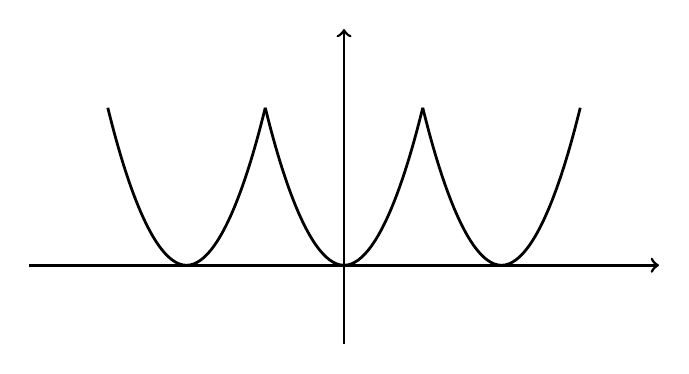
\begin{tikzpicture}[domain=1:5,line width=1pt]
\draw[->] (-4,0) -- (4,0);
\draw[->] (0,-1) -- (0,3);

\draw  (-3,2)  parabola  bend  (-2,0)  (-1,2);
\draw  (-1,2)  parabola  bend  (0,0)  (1,2);
\draw  (1,2)  parabola  bend  (2,0)  (3,2);
        
\end{tikzpicture}

$(2)按正弦展开,f(x)~\nsuminf \frac{(-1)^{n+1}}{n}sinnx-\frac{8}{\pi}\nsuminf \frac{sin(2n-1)x}{(2n-1)^2}$

\begin{tikzpicture}[domain=1:5,line width=1pt]
\draw[->] (-4,0) -- (4,0);
\draw[->] (0,-3) -- (0,3);

\draw[domain=-1:1] plot(\x,{tan(\x r)});

\draw[domain=1:3] plot(\x,{tan((\x-2) r)});

\draw[domain=-3:-1] plot(\x,{tan((\x+2) r)});
        
\end{tikzpicture}



$(3)在[0,2\pi]上展开,a_0=\frac{1}{\pi}\jf{0}{2\pi}f(x)dx=\frac{8}{3}\pi^2$

$a_n=\frac{1}{\pi}\jf{0}{2\pi}x^2cosnxdx=\frac{4}{n^2}$

$b_n=\frac{1}{\pi}\jf{0}{2\pi}x^2sinnxdx=-\frac{4\pi}{n}$

$f(x)~\frac{8}{3}\pi^2+4\nsuminf(\frac{cosnx}{n^2}-\pi \frac{sinnx}{n})$

\begin{tikzpicture}[domain=1:5,line width=1pt]
\draw[->] (-4,0) -- (4,0);
\draw[->] (0,-1) -- (0,3);

\draw[dashed] (1,0) -- (1,1.5);
\node [below] at (1,0) {2$\pi$};

\draw  (0,0)  parabola  (1,2);
        
\end{tikzpicture}

$\nl$

$例:设可积函数f(x)以2\pi 为周期,图形关于原点(\pm \frac{\pi}{2},0)对称,问$

$在(-\pi,\pi)的付氏系数有何特征?$

$f(x)=-f(-x) \to a_0=0,a_n=0,又有f(x)=-f(\pi-x)$

$b_n=\frac{2}{\pi} \jf{0}{\pi}f(x)sinnxdx=\frac{2}{\pi}(\jf{0}{\frac{\pi}{2}}f(x)sinnxdx+\jf{\frac{\pi}{2}}{\pi}f(x)sinnxdx)$

$=\frac{2}{\pi}(\jf{0}{\frac{\pi}{2}}f(x)sinnxdx+\jf{\frac{\pi}{2}}{0}-f(\pi-t)sinn(\pi-t)dt)$

$=\frac{2}{\pi} \jf{0}{\frac{\pi}{2}}f(x)sinnx(1+(-1)^n)dx$

$故b_{2n-1}=0$

$\nl$

$设f(x) \in R[-l,l]令t=\frac{\pi x}{l}则当x=[-l,l]时f \in [-\pi,\pi]于是$

$\phi(t) \triangleq f(\frac{lt}{\pi}) = f(t)在[-\pi,\pi]上可积,且$

$\phi(t) ~ \frac{a_0}{2}+ \sum(a_n cosnt+b_nsinnt)$

$a_n=\frac{1}{\pi}\jf{-\pi}{\pi}\phi (t)cosntdt$

$=\frac{1}{\pi} \frac{\pi}{l} \jf{-l}{l}f(x)cos \frac{n \pi x}{l}dx$

$b_n=\frac{1}{l}\jf{-l}{l}f(x)sin\frac{n\pi x}{l}dx$

$f(x)~\frac{a_0}{2}+\nsuminf (a_n cos\frac{n \pi x}{l}+b_n sin\frac{n \pi x}{l})$

$\nl$

$(1)f(x)为x到与它最近整数的距离$

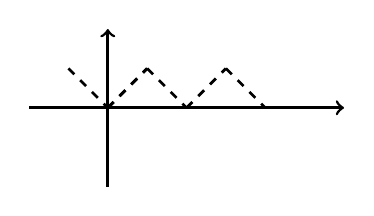
\begin{tikzpicture}[domain=1:5,line width=1pt]
\draw[->] (-1,0) -- (3,0);
\draw[->] (0,-1) -- (0,1);

\draw[dashed] (0,0) -- (0.5,0.5);
\draw[dashed] (-0.5,0.5) -- (0,0);

\draw[dashed] (0,0) -- (0.5,0.5);
\draw[dashed] (0.5,0.5) -- (1,0);

\draw[dashed] (1,0) -- (1.5,0.5);
\draw[dashed] (1.5,0.5) -- (2,0);


\end{tikzpicture}

$f(x)表示为偶函数,b_n=0,a_0=2\jf{0}{1}f(x)dx=\frac{1}{2}$

$a_n=2\jf{0}{1}f(x)cos2n\pi x=\frac{1}{(n\pi)^2}[(-1)^n-1],n \in N$

$a_{2n}=0,a_{2n-1}=-\frac{2}{\pi ^2} \frac{1}{(2n-1)^2}$

$f(x)~\frac{1}{4}-\frac{2}{\pi ^2}\nsuminf \frac{cos(2n-1)\pi x}{(2n-1)^2}$

$\nl$

$(2)f(x)=\begin{cases} e^x, 0 \le x < \frac{\pi}{2} \\ 0, -\frac{\pi}{2} \le x < 0 \end{cases} 在[-\frac{\pi}{2},\frac{\pi}{2}]上$

$a_0=\frac{2}{\pi}(e^{\frac{\pi}{2}}-1),a_n=\frac{1}{\pi} \frac{2}{1+4n^2}[(-1)^ne^{\frac{\pi}{2}}-1]$

$b_n=\frac{1}{\pi} \frac{4n}{1+4n^2}[(-1)^{n+1}e^{\frac{\pi}{2}}+1]$

$f(x)~\frac{1}{\pi}(e^{\frac{\pi}{2}}-1)+\frac{1}{\pi}\nsuminf  \frac{2}{1+4n^2}[(-1)^ne^{\frac{\pi}{2}}-1]cosnx+\nsuminf \frac{4n}{1+4n^2}[(-1)^{n+1}e^{\frac{\pi}{2}}+1] sinnx$

$= \begin{cases}  e^x,0<x<\frac{\pi}{2} \\ 0,-\frac{\pi}{2}<x<0  \\ \frac{1}{2}, x=0 \\  \frac{1}{2}e^{\frac{\pi}{2}},x=\pm \frac{\pi}{2}\end{cases}$

$\nl$

$Besel不等式,设f(x) \in R[-\pi,\pi],a_0,a_n,b_n是f(x)的付氏级数,则有$

$\frac{a_0}{2}+\nsuminf (a_n ^2+b_n^2) \le \frac{1}{\pi}\jf{-\pi}{\pi}f^2(x)dx$

$令S_n(x)=\frac{a_0}{2}+\ksum{1}{n}a_kcoskx+b_ksinkx$

$0 \le \jf{-\pi}{\pi}(f(x)-S_n(x))^2dx=\jf{-\pi}{\pi}f^2(x)dx-2\jf{-\pi}{\pi}f(x)S_n(x)dx+\jf{-\pi}{\pi}(S_n(x))^2dx$

$\jf{-\pi}{\pi}f(x)S_n(x)dx = \jf{-\pi}{\pi}f(x)(\frac{a_0}{2}+\ksum{1}{n}a_kcoskx+b_ksinkx)dx$

$=\frac{\pi}{2}a_0^2+\pi \nsuminf (a_k^2+b_k^2)$

$\jf{-\pi}{\pi}S_n(x)^2dx=\jf{-\pi}{\pi} \frac{a}{2}+\ksum{1}{n}a_kcoskx+b_ksinkx dx$

$=(\frac{a_0}{2})^2 \jf{-\pi}{\pi} dx= \ksum{1}{n} a_k^2 \jf{-\pi}{\pi}cos^2kxdx+b_k^2 \jf{-\pi}{\pi}sin^2kxdx$

$=\frac{\pi}{2}a_0^2+\ksum{1}{n}(a_k^2+b_k^2)$

$由上可知,当a_n,b_n为可积函数f(x)的付氏系数,必有a_n,b_n \to 0$

$\nl$

$设f(x)可积,且以2\pi 为周期,设S_n(x)为f(x)的付氏级数前2n+1项部分和,即$

$S_n(x)=\frac{a}{2}+\ksum{1}{n}(a_ncosnx+b_nsinnx)$

$则有S_n(x)=\frac{1}{\pi}\jf{0}{\pi}[f(x+t)-f(x-t)]\phi _n(t)dt$

$\nl$

$D_n(t)=\frac{sin(n+\frac{1}{2})t}{2sin\frac{t}{2}}称为Dirichlet核,D_n(0)=\frac{1}{2}$

$\nl$

$若f(x)在[a,b]只有有限个一类间断点,称为分散连续。若f(x),f'(x)在$

$[a,b]上分段连续,则f(x)在[a,b]上分段光滑.1·分段连续,分段光滑,函数均可积$

$对\forall x \in [a,b](广义)单侧导数存在,也即有$

$\ttx{0+}\frac{f(x+t)-f(x+0)}{t}=f'(x+0)$

$\ttx{0+}\frac{f(x-t)-f(x-0)}{t}=f'(x-0)$

$\nl$

级数

$\nl$

$例:设\{a_n\}单调递增且恒正,证明级数\nsuminf \frac{a_n-a_{n-1}}{a_na_{n-1}^ \lambda}(\lambda > 0)收敛$

$(1)\ntinf a_n=a,0 \le  \frac{a_n-a_{n-1}}{a_na_{n-1}^ \lambda} \le  \frac{a_n-a_{n-1}}{a_{0}^ {\lambda+1}}=k(a_n-a_{n-1}), \forall n \in N$

$(2)\ntinf a_n=\infty,0 \le  \frac{a_n-a_{n-1}}{a_na_{n-1}^ \lambda}=\frac{1}{a_{n-1}^\lambda}-\frac{1}{a_na_{n-1}^{\lambda-1}} \le \frac{1}{a_{n-1}^\lambda}-\frac{1}{a_{n}^\lambda}$

$\nl$

$给定\nsuminf \frac{a_n}{n^x},其中a_n \in N,证明:\exists r(-\infty \le r \le +\infty)使得当x<r$

$时级数发散,x>r时级数收敛$

$先证:\sum \frac{a_n}{n^ \lambda}收敛,则\forall x>\lambda,\sum \frac{a_n}{n^x}必收敛(Abel)$

$再证r存在,对\forall x \in R,\sum \frac{a_n}{n^x}恒收敛或恒发散,则r=\pm \infty$

$不妨设x_1使得\sum \frac{a_n}{n^{x_1}}发散,x_2使得\sum \frac{a_n}{n^{x_2}}收敛,由前面$

$证有x_1<x_2,记E=\{x|\nsuminf \frac{a_n}{n^x}收敛\}$

$记r=infE,若r \in R,则证毕,若r \notin E,则存在$

$单调递减\{x_n\} \subset E,x_n \to r,存在充分大n,使得x_n < x,也有$

$x \in E,若x<r,则x \notin E,\sum \frac{a_n}{n^x}必发散$

$\nl$

$若对于任何一个收敛于0的数列\{x_n\},\sum a_n x_n都收敛,证明$

$ \sum a_n 绝对收敛$

$反证法,若\nsuminf |a_n|发散,即\forall n,k \in N,\exists m(m>n) \isum{1}{m}|a_i| \ge k$

$对n=1,k=1,\exists m_1 \in N:\isum{1}{m_1}|a_i| \ge 1$

$对n=m_1+1,k=2,\exists m_2 \ge m_1+1,\isum{m_1+1}{m_2}|a_i| \ge 2$

$对1 \le m_1 \le m \le ... m_k \le ... 使\isum{m_{k-1}}{m_k}|a_i| \ge k,k=1,2,3...$

$取x_i = \frac{1}{k} sgn a_i(n_{k-1} \le i \le m_k)则对\forall N>0,只要k-1 >N$

$总有m_k>m_{k-1}>N,此时 \isum{m_{k-1}+1}{n_k}a_i x_i = \isum{m_{k-1}+1}{m_k} \frac{|a_i|}{k} \ge 1,不满足条件$

$\nl$

$例:设正项级数\nsuminf a_n收敛,证明: \ptx{+\infty}(\nsuminf a_n^p)^{\frac{1}{p}} = sup(a_n)$

$由正项级数\nsuminf a_n收敛,必有 \ntinf a_n =0,故\exists N:0<a_n<a_1,\forall n>N$

$故sup\{a_n\}=max(a_1,a_2,...a_N)记为a_{n_0}=max(a_1,a_2,...a_N)$

$(1 \le n_0 \le N),则有a_{n_0}=sup_n \{a_n\}$

$又有p\to +\infty,令p>1,则当n充分大时,总有a_n^P<a_n,由$

$\nsuminf a_n 收敛,故\nsuminf a_n^p也收敛,于是由收敛定义可知\exists N:$

$\nsum{N+1}{\infty}a_n^P<a_{n_0}^P,于是有a_{n_0}=(a_{n_0}^P)^{\frac{1}{p}} \le (\nsuminf a_n^P)^{\frac{1}{p}} = (\nsum{1}{r} a_n^P + \nsum{r+1}{\infty} a_n^P)^{\frac{1}{p}}$ 

$\le (\nsum{1}{r} a_n^P + a_{n_0}^P)^{\frac{1}{p}} \le (Na_{n_0}^P + a_{n_0}^P)^{\frac{1}{p}} = ((N+1)a_{n_0}^P)^{\frac{1}{p}}$

$(N+1)^{\frac{1}{p}}a_{n_0}$

$\nl$

$证明:任何有理数必为调和级数中有限项之和$

$设\frac{A}{B}为正有理数,A,B \in N,因为\sum \frac{1}{n}发散,故\exists n_0 \in N:$

$\ksum{1}{n} \frac{1}{k} \le \frac{A}{B}  < \ksum{1}{n+1} \frac{1}{k}$

$若等式不成立,作新有理数\frac{C}{D}=\frac{A}{B}-\ksum{1}{n},则\frac{C}{D}< \frac{1}{n_0+1}$

$又\exists n_1 \in N, \frac{1}{n_1+1} \le \frac{C}{D} < \frac{1}{n_1},若等号不成立,作\frac{E}{F}= \frac{C}{D} - \frac{1}{n_1+1} >0$

$\exists n_2 \in N, \frac{1}{n_2+1} \le \frac{E}{F} < \frac{1}{n_2}....$

$由上有\frac{A}{B} > \frac{C}{D} > \frac{E}{F}...且C>E>.... $

$\frac{C}{D} - \frac{1}{n+1} = \frac{(n+1)C-D}{D(n+1)} = \frac{C-\frac{D}{n+1}}{D} \triangleq \frac{E}{F},C-E=C-[(n+1)C-D]=D-nC>0$

$上述分子经过有限步运算后减为1,....$

$\nl$

$设\{a_n\}满足a_n=\ksuminf tg^2a_{n+k},n \in N,若\nsuminf a_n收敛,a_n \equiv 0$

$改写条件为a_n= \msum{n+1}{\infty}tg^2a_m,可知\{a_n\}单调递减非负$

$又由\xtx{0+}\frac{tgx}{x}=1,\exists \epsilon_0(0<\epsilon_0 \le \frac{1}{\delta}),tgx<2x,\forall x \in [0,\epsilon_0]$

$由\nsuminf a_n 收敛,故\exists N \in \bold N : \nsum{N+1}{\infty}a_n < \epsilon_0 \le \frac{1}{\delta}$

$此时必有a_n \le \epsilon_0,\forall n \ge N+1,于是由上式可得$

$tga_n < 2a_n \to tg^a_n < 4a_n^2,\forall n>N$

$从而,a_N=\nsum{N+1}{\infty}tg^2a_n \le \nsum{N+1}{\infty} 4a_n^2 \le 4\nsum{N+1}{\infty}a_Na_n \le 4 \epsilon_0 a_N \le \frac{a_N}{2}$

$a_N=0,故由a_n单调递减非负,可令a_n \equiv 0,n>N$

$由a_{N-1}=\nsum{N}{\infty}tg^2a_n=0,a_{N-2}=0,...$

$\nl$

$设f_n(x)(n \in N)为[a,b]上的单调函数,\ntinf f_n(x)=f(x),且f(x) \in C[a,b]$

$证明:\{f_n(x)\}在[a,b]上一致收敛$

$(5 \epsilon 法)等分区间$

$\nl$

$设可微函数列\{f_n(x)\}在[a,b]上收敛,\{f_n'(x)\}在[a,b]上一致有界$

$证明\{f_n(x)\}在[a,b]上一致收敛$

$证法1:设|f'_n(x)| \le M,\forall n \forall x,对\forall \epsilon >0,对[a,b]作分法T,$

$a=x_0 < x_1 <..x_p=b,max|x_k-x_{k-1}|< \frac{\epsilon}{3M}对\forall x \in(a,b)总有$

$k(0 \le k \le p)x \in[x_{k-1},x_k],中值定理$

$|f_n(x)-f_n(x_k)|=|f'_n(\zeta)|·|x-x_k|< M \frac{\epsilon}{3M} \le \frac{\epsilon}{3}$

$于是有|f_n(x)-f_m(x)| \le |f_n(x)-f_n(x_k)|+|f_n(x_k)-f_m(x_k)|+|f_m(x_k)-f_m(x)|$

$已知\{f_n(x_k)\}收敛,\exists N_k \in N$

$|f_m(x_k)-f_n(x_k)|<\frac{\epsilon}{3},\forall m,n>N_k$

$取N=max(N_k,...N_p),|f_n(x)-f_m(x)|< \frac{\epsilon}{3}+\frac{\epsilon}{3}+\frac{\epsilon}{3}=\epsilon. \forall m,n>N,\forall x$

$\nl$

$证法二:有限覆盖定理,\forall \epsilon > 0,\forall x \in [a,b],\exists N',-N'(\epsilon,x')$

$|f_m(x')-f_n(x')|<\frac{\epsilon}{2},\forall m,n>N',记|f_n'(x)|\le M,\forall n \in N$

$\forall x \in[a,b],取\delta'=\frac{\epsilon}{4M},则对\forall x \in \cup(x',\delta')有|f_m(x)-f_n(x)|$

$\le |f_m(x)-f_m(x')|+|f_m(x')-f_n(x')|+|f_n(x')-f_n(x)| \le$

$2m|x-x'|+|f_m(x')-f_m(x')|<2M\frac{\epsilon}{4M}+\frac{\epsilon}{2}=\epsilon$

$上式对m,n>N',\forall x \in \cup(x',\delta')均成立,记G=\{\cup(x',\delta')|\forall x' \in[a,b]\}$

$则G为[a,b]开覆盖$

$\nl$

$设\nsuminf u_n(x)在[a,b]上有和函数S(x),又u_n(x) \in C[a,b],且非负$

$(n\in N),证明S(x)在[a,b]上可达最小值$

$因为u_n(x)\ge 0,故S(x) \ge 0,于是m=inf\{S(x)|x \in(a,b)\}存在$

$若有x^* \in[a,b],S(x^*)=m命题成立,否则\exists \{x_i\} \subset$

$[a,b]设\itinf S(x_i)=m,由于\{x_i\}有界,必有收敛子列,$

$因为\nsuminf u_n(x_0)=S(x_0),\forall \epsilon >0,\exists N \in \bold N:|\nsum{1}{N}u_n(x_0)-S(x_0)|<\frac{\epsilon}{2}$

$\to \nsum{1}{N}u_n(x_0)>S(x_0)-\frac{\epsilon}{2},由\nsum{1}{N}u_n(x)在x_0连续,对上述\epsilon$

$>0,\exists \delta>0,对\forall x(|x-x_0|<\delta):|\nsum{1}{N}u_n(x)-\nsum{1}{N}u_n(x_0)|<\frac{\epsilon}{2}$

$也即有\nsum{1}{N}u_n(x)>\nsum{1}{N}u_n(x_0)-\frac{\epsilon}{2},因为x_i\to x_0(i \to \infty)$

$故\exists I_0,当i>I_0时有|x_i-x_0|<\delta,于是有$

$\nsum{1}{N}u_n(x_i)>\nsum{1}{N}u_n(x_0)-\frac{\epsilon_0}{2}>S(x_0)-\frac{\epsilon}{2}-\frac{\epsilon}{2}=S(x_0)-\epsilon$

$由于u_n(x) \ge 0(\forall n \in N)所以S(x_i) \ge \nsum{1}{N}u_n(x_i) > S(x_0)- \epsilon$

$取极限有\itinf S(x_i) \ge S(x_o)-\epsilon  \to m>S(x_0)-\epsilon$

$m \le S(x_0) \le m+\epsilon$

$S(x)在[a,b]上未必达到最大值$

$u_n(x)=(1-x)x^n,x \in[0,1]$

$可以u_n(x) \ge 0,m(x) \in C[0,1],\forall n \in N,S(x)=\begin{cases} x \\ 0 \end{cases}$

$\nl$

$定理1,设f(x)以2\pi 为周期,在[-\pi,\pi]上分段光滑,则f(x)的付氏级数$

$收敛,且有\frac{1}{2}(f(x+0)-f(x-0))=\frac{a}{2}+\sum(a_ncosnx+b_nsinnx)$

$\nl$

$f(x)=x^2(0<x<2\pi)展开付氏级数,由此计算\sum \frac{1}{n^2},\sum \frac{(-1)^{n+1}}{n^2},\nsuminf \frac{1}{(2n-1)^2}$

$余弦展开f(x)~\frac{\pi ^2}{2}+4\sum \frac{(-1)^n}{n^2}cosnx=x^2$

$令x=\pi,则有\sum \frac{1}{n^2}=\frac{\pi^2}{6}$

$正弦展开f(x)~\frac{4\pi^2}{3}+4\nsuminf \frac{cosnx}{n^2}-4\pi\nsuminf \frac{sinnx}{n}$

$令x=\pi,得\sum \frac{(-1)^{n+1}}{n^2}=\frac{\pi^2}{12}$

$以上两式相加2\nsuminf \frac{1}{(2n-1)^2}=\frac{\pi^2}{4}$

$\nl$

$广义的牛顿莱布尼兹公式,设f(x)\in C[a,b]且分段光滑,则有$

$\jf{a}{b}f'(x)dx = f(b)-f(a)$

$广义分部积分公式:\jf{a}{b}f'(x)sin \lambda x dx=f(x)sin \lambda x|_a^b \pm \lambda \jf{a}{b}f(x)cos \lambda xdx$

$\jf{a}{b}f'(x)cos \lambda x dx=f(x)cos \lambda x|_a^b \pm \lambda \jf{a}{b}f(x)sin \lambda xdx$

$\nl$

$设f(x) \in C \bold R,以2\pi 为周期,且在[-\pi,\pi]上分段光滑,则f(x)付氏系数在R上一致收敛$

$\nl$

$周期为2\pi,f(x)=\frac{1}{4}x(2\pi-x),x \in [0,2\pi]$

$f(x)~\frac{1}{6}\pi^2-\nsuminf \frac{1}{n^2}cosnx,令x=0,\sum \frac{1}{n^2}=\frac{\pi^2}{6}$

$对付氏系数逐项积分,\frac{1}{4}(\pi x^2-\frac{x^3}{3})=\frac{1}{6}\pi^2 x- \nsuminf \frac{1}{n^3}sinnx$

$令x=\frac{\pi}{2},\nsuminf \frac{(-1)^{n-1}}{(2n-1)^3}=\frac{1}{32}\pi^3$

$再积分\frac{1}{4}(\frac{\pi x^3}{3}-\frac{x^4}{12})=\frac{1}{12}\pi^2x^2+\nsuminf \frac{1}{n^4}(cosnx-1)$

$再积分\frac{1}{4}(\frac{\pi x^4}{12}-\frac{x^5}{60})=\frac{1}{36}\pi^2x^3+\nsuminf(\frac{sinnx}{n}-x)$

$令x=2\pi,\nsuminf \frac{1}{n^4}=\frac{\pi^4}{90}$

$\nl$

$Parseral等式,设可积函数f(x)的付氏系数在[-\pi,\pi]上的一致收敛,则有$

$\frac{1}{\pi} \jf{-\pi}{\pi}f(x)^2dx = \frac{a_0^2}{2}+\nsuminf (a_n^2+b_n^2)$

$f(x)=x(\pi-x),0<x<\pi,正弦展开,并计算\sum \frac{1}{n^6}$

$延拓f=\begin{cases}x(\pi-x),0\le x<\pi \\ x(\pi+x), -\pi<x\le0 \end{cases}$

$f(x)=\frac{8}{\pi}\nsuminf \frac{sin(2n-1)x}{(2n-1)^3},-\pi \le x \le \pi,b_{n-1}=\frac{8}{\pi}\frac{1}{(2n-1)^3}$

$由Parscal等式,\frac{1}{15}\pi^4=\frac{1}{\pi}\jf{-\pi}{\pi}f^2(x)dx=\nsuminf b_n^2=\frac{64}{\pi}\nsuminf \frac{1}{(2n-1)^6}$

$从而\nsuminf \frac{1}{(2n-1)^6}=\frac{\pi^6}{64·15}故有\sum \frac{1}{n^6}=\frac{\pi^6}{945}$

$\nl$

$设f(x) \in C(R),以2\pi 为周期,在[-\pi,\pi]上分段光滑,g(x)\in R[-\pi,\pi]$

$则有\frac{1}{\pi}\jf{-\pi}{\pi}f(x)g(x)dx=\frac{a_0\alpha_0}{2}+\nsuminf(a_n\alpha_n+b_n\beta_n)$

$证明:f(x)在R上连续周期为2\pi ,分段光滑$

$\frac{1}{2}a_0+\nsuminf(a_ncosnx+b_nsinnx) \to ^{[-\pi,\pi]} f(x)$

$g(x)可积,|g(x)|\le M,\forall x \in [-\pi,\pi]$

$|\frac{1}{\pi}\jf{-\pi}{\pi}f(x)g(x)-\frac{1}{\pi}\jf{-\pi}{\pi}g(x)(\frac{1}{2}a_0+\sum a_k coskx+b_k sinx dx)|$

$\le \frac{1}{2} \jf{-\pi}{\pi} |g(x)||f(x)|-|\frac{1}{2}a_0+\sum |a_k coskx+b_k sinkx|dx$

$证法2:f·g= \frac{a_0}{2}g+\sum(a_k coskx+b_k sinkx)g$

$逐项积分,即有.......$

$证法三:f(x)\pm g(x)的减弱的Pasacal等式....消去平方项$

$\nl$

$函数逼近论$

$定理1,设f(x) \in C[a,b],则\forall \epsilon > 0,存在分段光滑函数L(x)使得$

$|f(x)-L(x)| < \epsilon, \forall x \in [a,b]$

$\nl$

$第一逼近定理,设f(x) \in CR,以2\pi 为周期,则\forall \epsilon >0,存在三角多项式$

$T_n(x)=\frac{a_0}{2}+\ksuminf (a_k coskx+b_k sinkx)$

$使得当n充分大时候有 |f(x)-T_n(x)|< \epsilon, \forall x \in R$

$\nl$

$第二逼近定理f(x) \in C[a,b] \forall \epsilon >0,存在多项式P_n(x),|f-P_n|< \epsilon,\forall x$

$例:f(x)的k次矩定义为\jf{a}{b}f(x)x^kdx,k=0,1,2,.....若f(x) \in C[a,b]$

$且f(x)的一切k次矩为0,则f(x)=0$

$\forall \epsilon >0,\exists P_n(x):|f-P_n|< \epsilon$

$\jf{a}{b}fP_ndx=\jf{a}{b}f(x)(a_0+a_1x+...a_nx^n)dx=0$

$于是\jf{a}{b}f^2(x)dx = \jf{a}{b}f(x)[f(x)-P_n(x)]dx+\jf{a}{b}f(x)P_n(x)dx(=0)$

$=\jf{a}{b}f(x)|f(x)-P_n(x)|dx \le |f(x)-P_n(x)|\jf{a}{b}f(x)dx$

$\epsilon \jf{a}{b}f(x)dx \triangleq M\epsilon$

$\nl$

$n!=\sqrt{2\pi n}n^n e^{-n+\frac{\theta_n}{12n}}(0<\theta_n<1)$

$\nl$

$设f(x) \in C[0,1]令P_n(x)=\frac{1}{I_n}\jf{0}{1}f(v)[1-(v-x)^2]^ndv为2n次多项式$

$I_n=\jf{-}{1}(1-n^2)^ndn,P_n(x) \to f(x)$

\end{document}

